\paragraph{QuizziPedia::Front-End::ModelViews::HomeModelView}
	
	\label{QuizziPedia::Front-End::ModelViews::HomeModelView}
	
	\begin{figure}[ht]
		\centering
		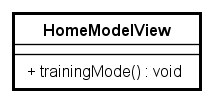
\includegraphics[scale=0.80,keepaspectratio]{UML/Classi/Front-End/QuizziPedia_Front-end_ModelView_HomeModelView.png}
		\caption{QuizziPedia::Front-End::ModelViews::HomeModelView}
	\end{figure} \FloatBarrier
	
	\begin{itemize}
		\item \textbf{Descrizione}: classe di tipo modelview la cui istanziazione è contenuta all'interno della variabile di ambiente \texttt{\$scope} di \textit{Angular\ped{G}}. All'interno di essa sono presenti le variabili e i metodi necessari per il \textit{Two-Way Data-Binding\ped{G}} tra la \textit{view\ped{G}} \texttt{HomeView} e il \textit{controller\ped{G}} \texttt{HomeController};
		\item \textbf{Utilizzo}: viene utilizzata per effettuare il \textit{Two-Way Data-Binding\ped{G}} tra la \textit{view\ped{G}} \texttt{HomeView} e il \textit{controller\ped{G}} \texttt{HomeController} rendendo disponibili variabili e metodi;
		\item \textbf{Relazioni con altre classi}: 
		\begin{itemize}
			\item \textbf{OUT \texttt{HomeView}}: \textit{view\ped{G}} contenente la direttiva per barra di ricerca degli utenti e questionari e il bottone che porterà l'utente nella modalità allenamento; 
			\item \textbf{OUT \texttt{HomeController}}: questa classe permette di gestire la home page;
		\end{itemize}
		\item \textbf{Metodi}: 
		\begin{itemize}
			\item \texttt{+ trainingMode(): void} \\
			Metodo che gestisce l’evento click sul pulsante di allenamento. Effettua il redirect alla pagina di allenamento.
			\item \texttt{+} \texttt{search(): void} \\
			Metodo che gestisce l’evento click sul pulsante di ricerca. Effettua il redirect alla pagina di ricerca passando come parametro la stringa digitata.
		\end{itemize}
	\end{itemize}
	
	